\section*{Introduction}\index{Neuropterida}
Neuropterida is comprised of three orders---\textbf{Neuroptera} \textit{sensu stricto}, \textbf{Megaloptera}, \textbf{Raphidioptera}---that are occasionally treated as one: Neuroptera \textit{sensu lato}. The common ancestor of these insects is almost definitely a predator, as almost all extant species eat other metazoans. There are several larval characters that support the monophyly of this lineage, the most interesting of which, perhaps, is the piercing-sucking, sickle-shaped mandibles with the maxillary groove and associated venom glands. These insects are less diverse (\textless7,000 extant species) than other holometabolans, although the fossil record suggests they were \textit{much} more diverse in the past. The sister lineage to Neuropterida is likely the branch containing Coleoptera and Strepsiptera.

\section{Megaloptera}\index{Megaloptera}
The larvae of all species develop in aquatic habitats;
 hind wings broader at base than fore wings; the hind wings with expanded anal lobes and extra anal veins.\vspace{3mm}

\subsubsection{Corydalidae (Dobsonflies, fishflies)}\index{Corydalidae}

\noindent{}\textit{Diagnostic characters:} Body usually large to very large (\textgreater25 mm); ocelli present; tarsomere 4 cylindrical; wings rarely completely dark.\vspace{3mm}

\noindent{}\textit{Natural history:} Larvae (hellgrammites) develop as generalist predators of aquatic insects, mainly in lotic habitats. Adults probably do not feed. Males usually have long, curved mandibles that are used in courtship and in fighting other males. Just over 200 species have been described worldwide.\vspace{3mm}

\begin{figure}[ht!]
  \centering
    \includegraphics[width=0.65\textwidth]{neuropterida/CorydalidHabitus}
\caption{Corydalidae habitus \citep[modified from][Fig. 56c,d]{walsh2004hellgrammite}}
  \label{fig:corydalid}
\end{figure}

\subsubsection{Sialidae (alderflies)}\index{Sialidae}
\noindent{}\textit{Diagnostic characters:} Body usually medium sized (\textless25 mm); ocelli absent; tarsomere 4 bilobed; wings usually entirely dark, almost black in color.\vspace{3mm}

\noindent{}\textit{Natural history:} Fewer than 100 species have been described worldwide, all of which are thought to be generalist predators of aquatic invertebrates in lotic environments.\vspace{3mm}

\begin{figure}[ht!]
  \centering
    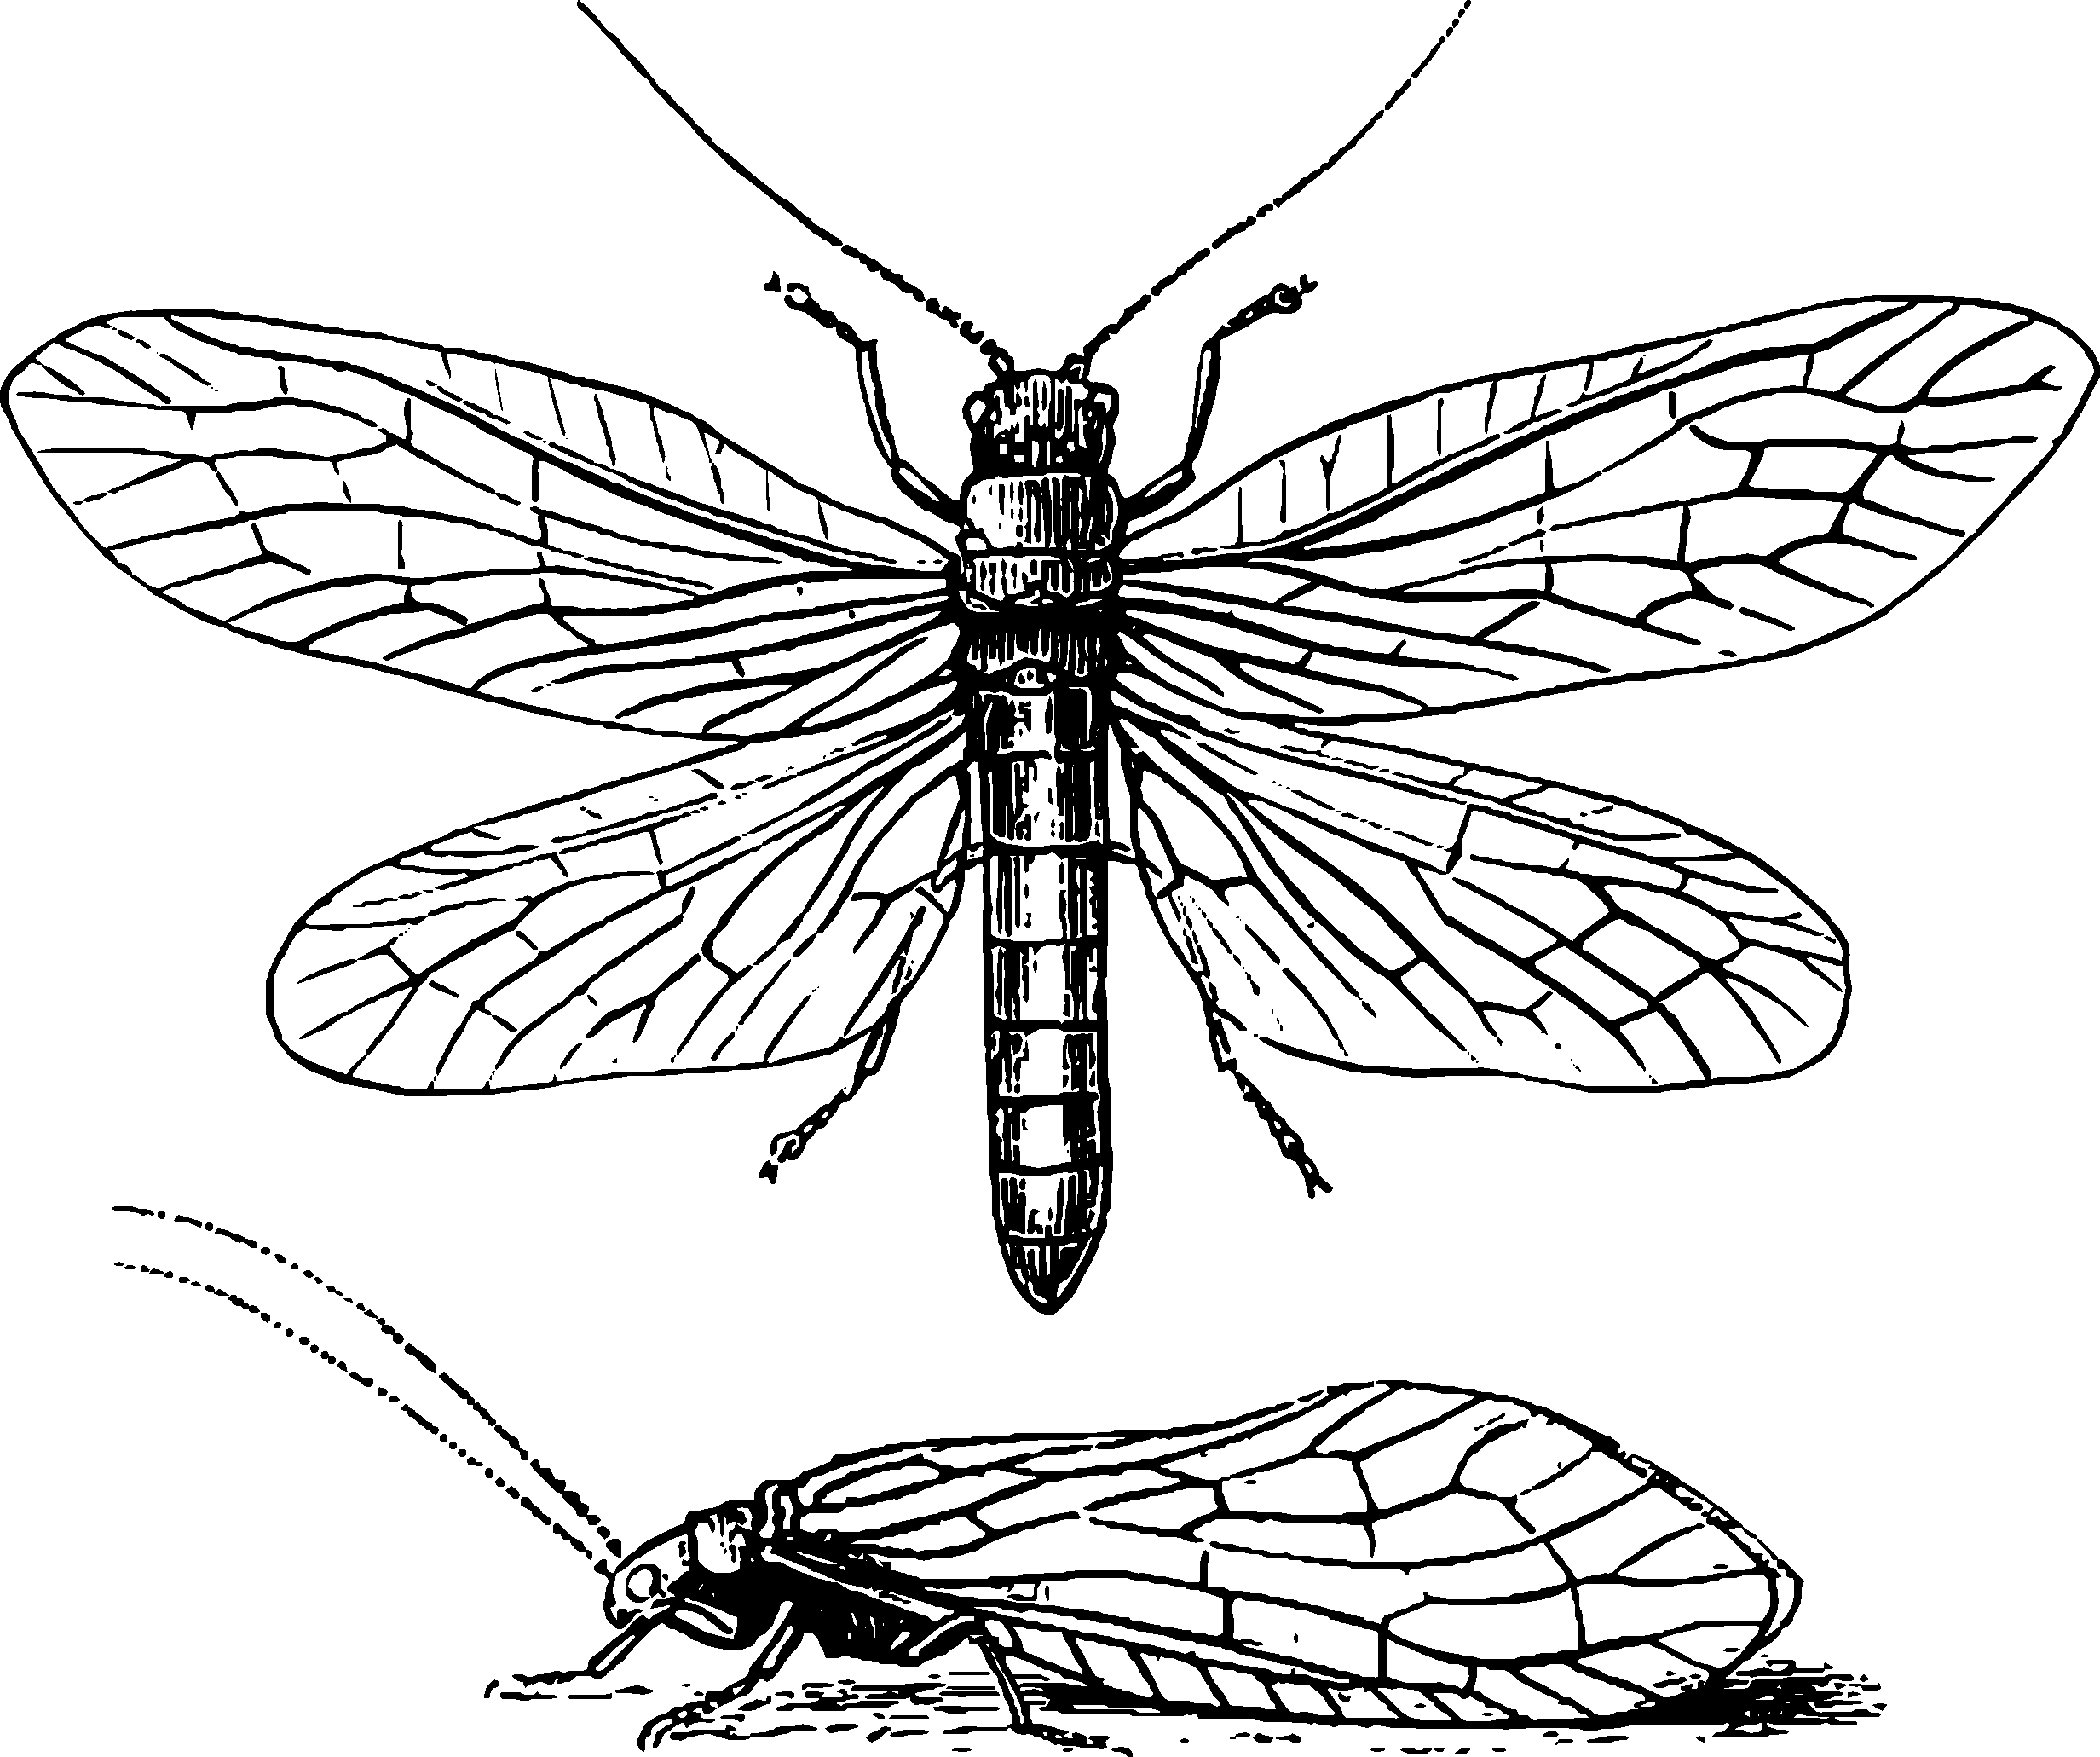
\includegraphics[width=0.45\textwidth]{neuropterida/sialidae}
  \caption{Sialidae \citep[modified from Fig. 286 in][]{bhlitem56570}}
  \label{fig:sialid1}
\end{figure}

\begin{theo}
{}Megaloptera have many of the same key innovations as other Holometabola, including dicondylous mandibles, neopteran wings, and complete development. Why are there several orders of magnitude fewer species than, say, Hymenoptera?
\end{theo}

\section{Neuroptera}\index{Neuroptera}
Lacewings typically have complex wing venation and similarly shaped fore and hind wings, superficially similar to Odonata (with which they were classified a long time ago). Larvae of most species are terrestrial, have a closed gut, and almost all predate on other invertebrates. More than 6,000 species have been described worldwide.\vspace{3mm}

\subsubsection{Sisyridae (spongillaflies)}\index{Sisyridae}
\noindent{}\textit{Diagnostic characters:} Wings gray to brown, sometimes patterned; wings with few cross veins except along anterior margin; most of these crossveins are not forked. The subcosta (Sc) and radius (R1) meet near the wing apex.\vspace{3mm}

\noindent{}\textit{Natural history:} These uncommon lacewings are usually collected near aquatic habitats, where the larvae live as predators of freshwater sponges. There are fewer than 10 species in North America and only about 60 worldwide.\vspace{3mm}

\begin{figure}[ht!]
    \centering
    \begin{subfigure}[ht!]{0.31\textwidth}
      \centering
        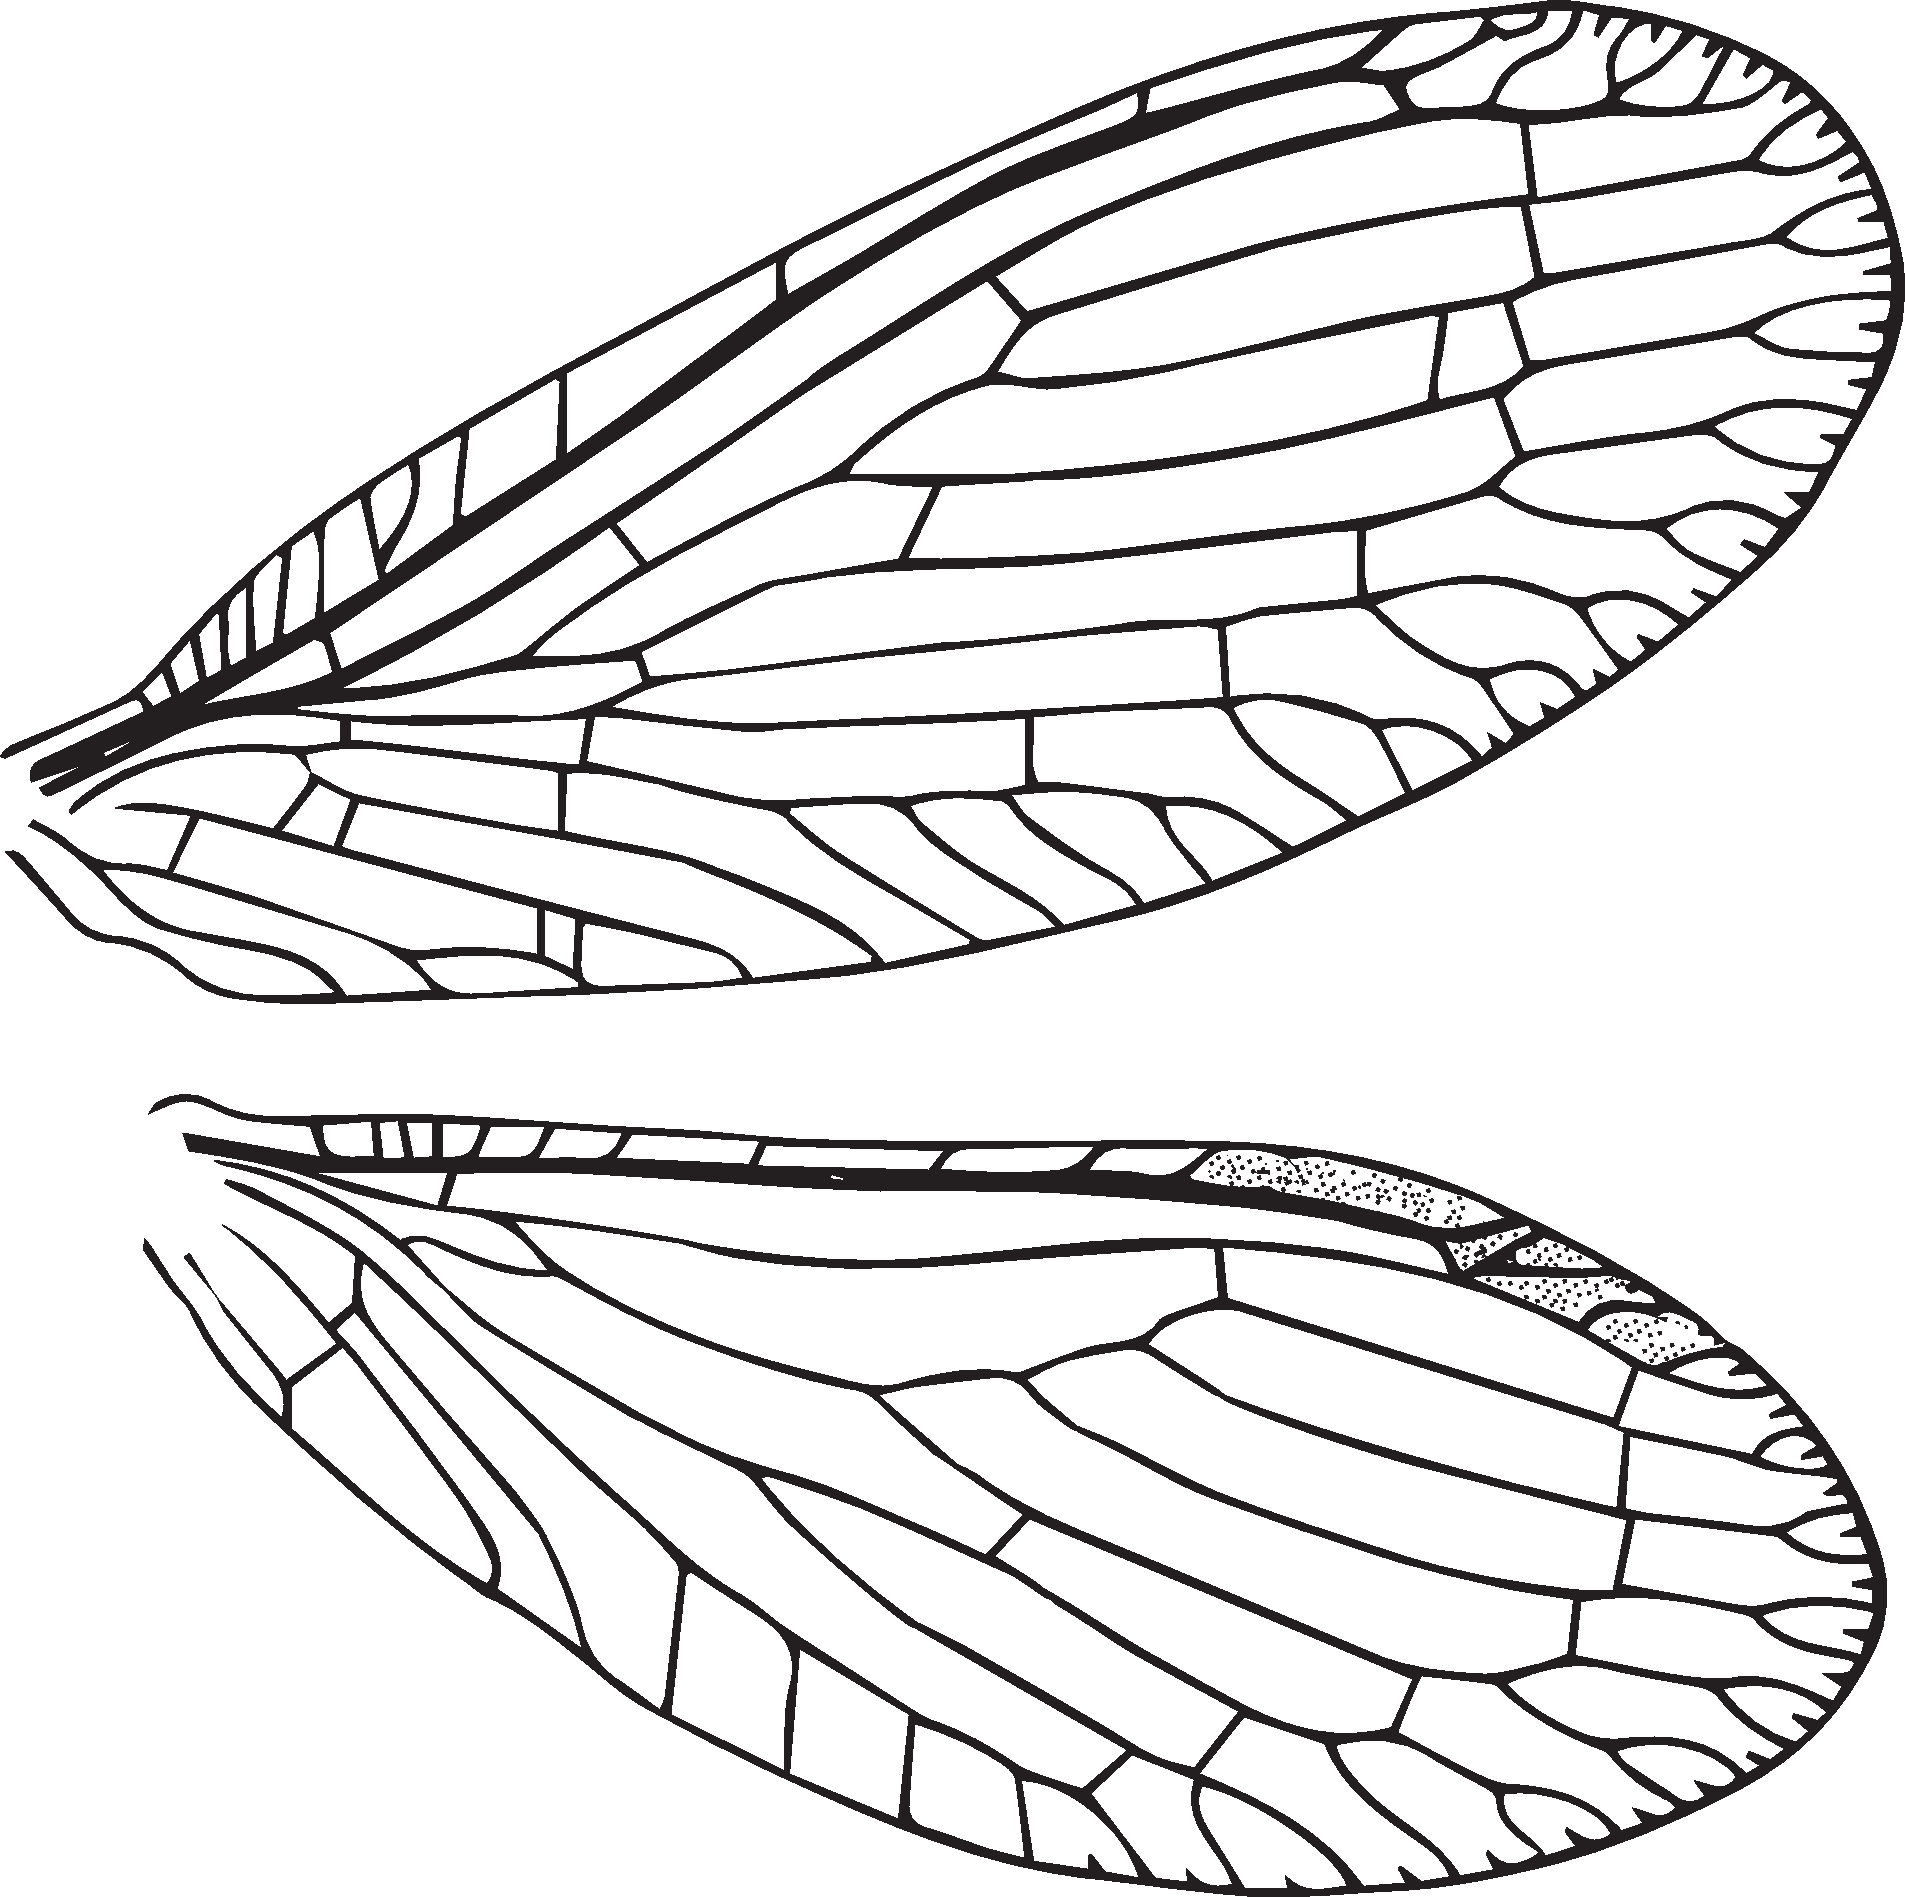
\includegraphics[width=\textwidth]{neuropterida/sisyridWings}
        \caption{}
        \label{fig:sisyrid}
    \end{subfigure}
    \hfill
    \begin{subfigure}[ht!]{0.55\textwidth}
        \includegraphics[width=\textwidth]{neuropterida/sisyridHabitus}
        \caption{}
        \label{fig:sisyrid2}
    \end{subfigure}
    \caption{Sisyridae. \textbf{(a)} Wings \citep[][Fig. 328]{bhl29907}; \textbf{(b)} Habitus, photo (CC BY 2.0) by Auckland Museum \url{https://bit.ly/363DaPj} }\label{fig:sisyrids}
\end{figure}

\subsubsection{Myrmeleontidae (ant lions)}\index{Myrmeleontidae}
\noindent{}\textit{Diagnostic characters:} Antenna as long as head + thorax; apical flagellomeres wider than proximal antennomeres; eyes never divided horizontally; thorax setose but not especially ``fuzzy''.\vspace{3mm}

\noindent{}\textit{Natural history:} Larvae develop as ambush predators in terrestrial environments, with many species (but not all!) digging conical pits in loose substrates (\textit{e.g.}, fine-grained sand) to trap prey. Many adults likewise feed on other insects, although some are also known to eat pollen. Almost 2,000 species are known worldwide.\vspace{3mm}

\begin{figure}[ht!]
  \centering
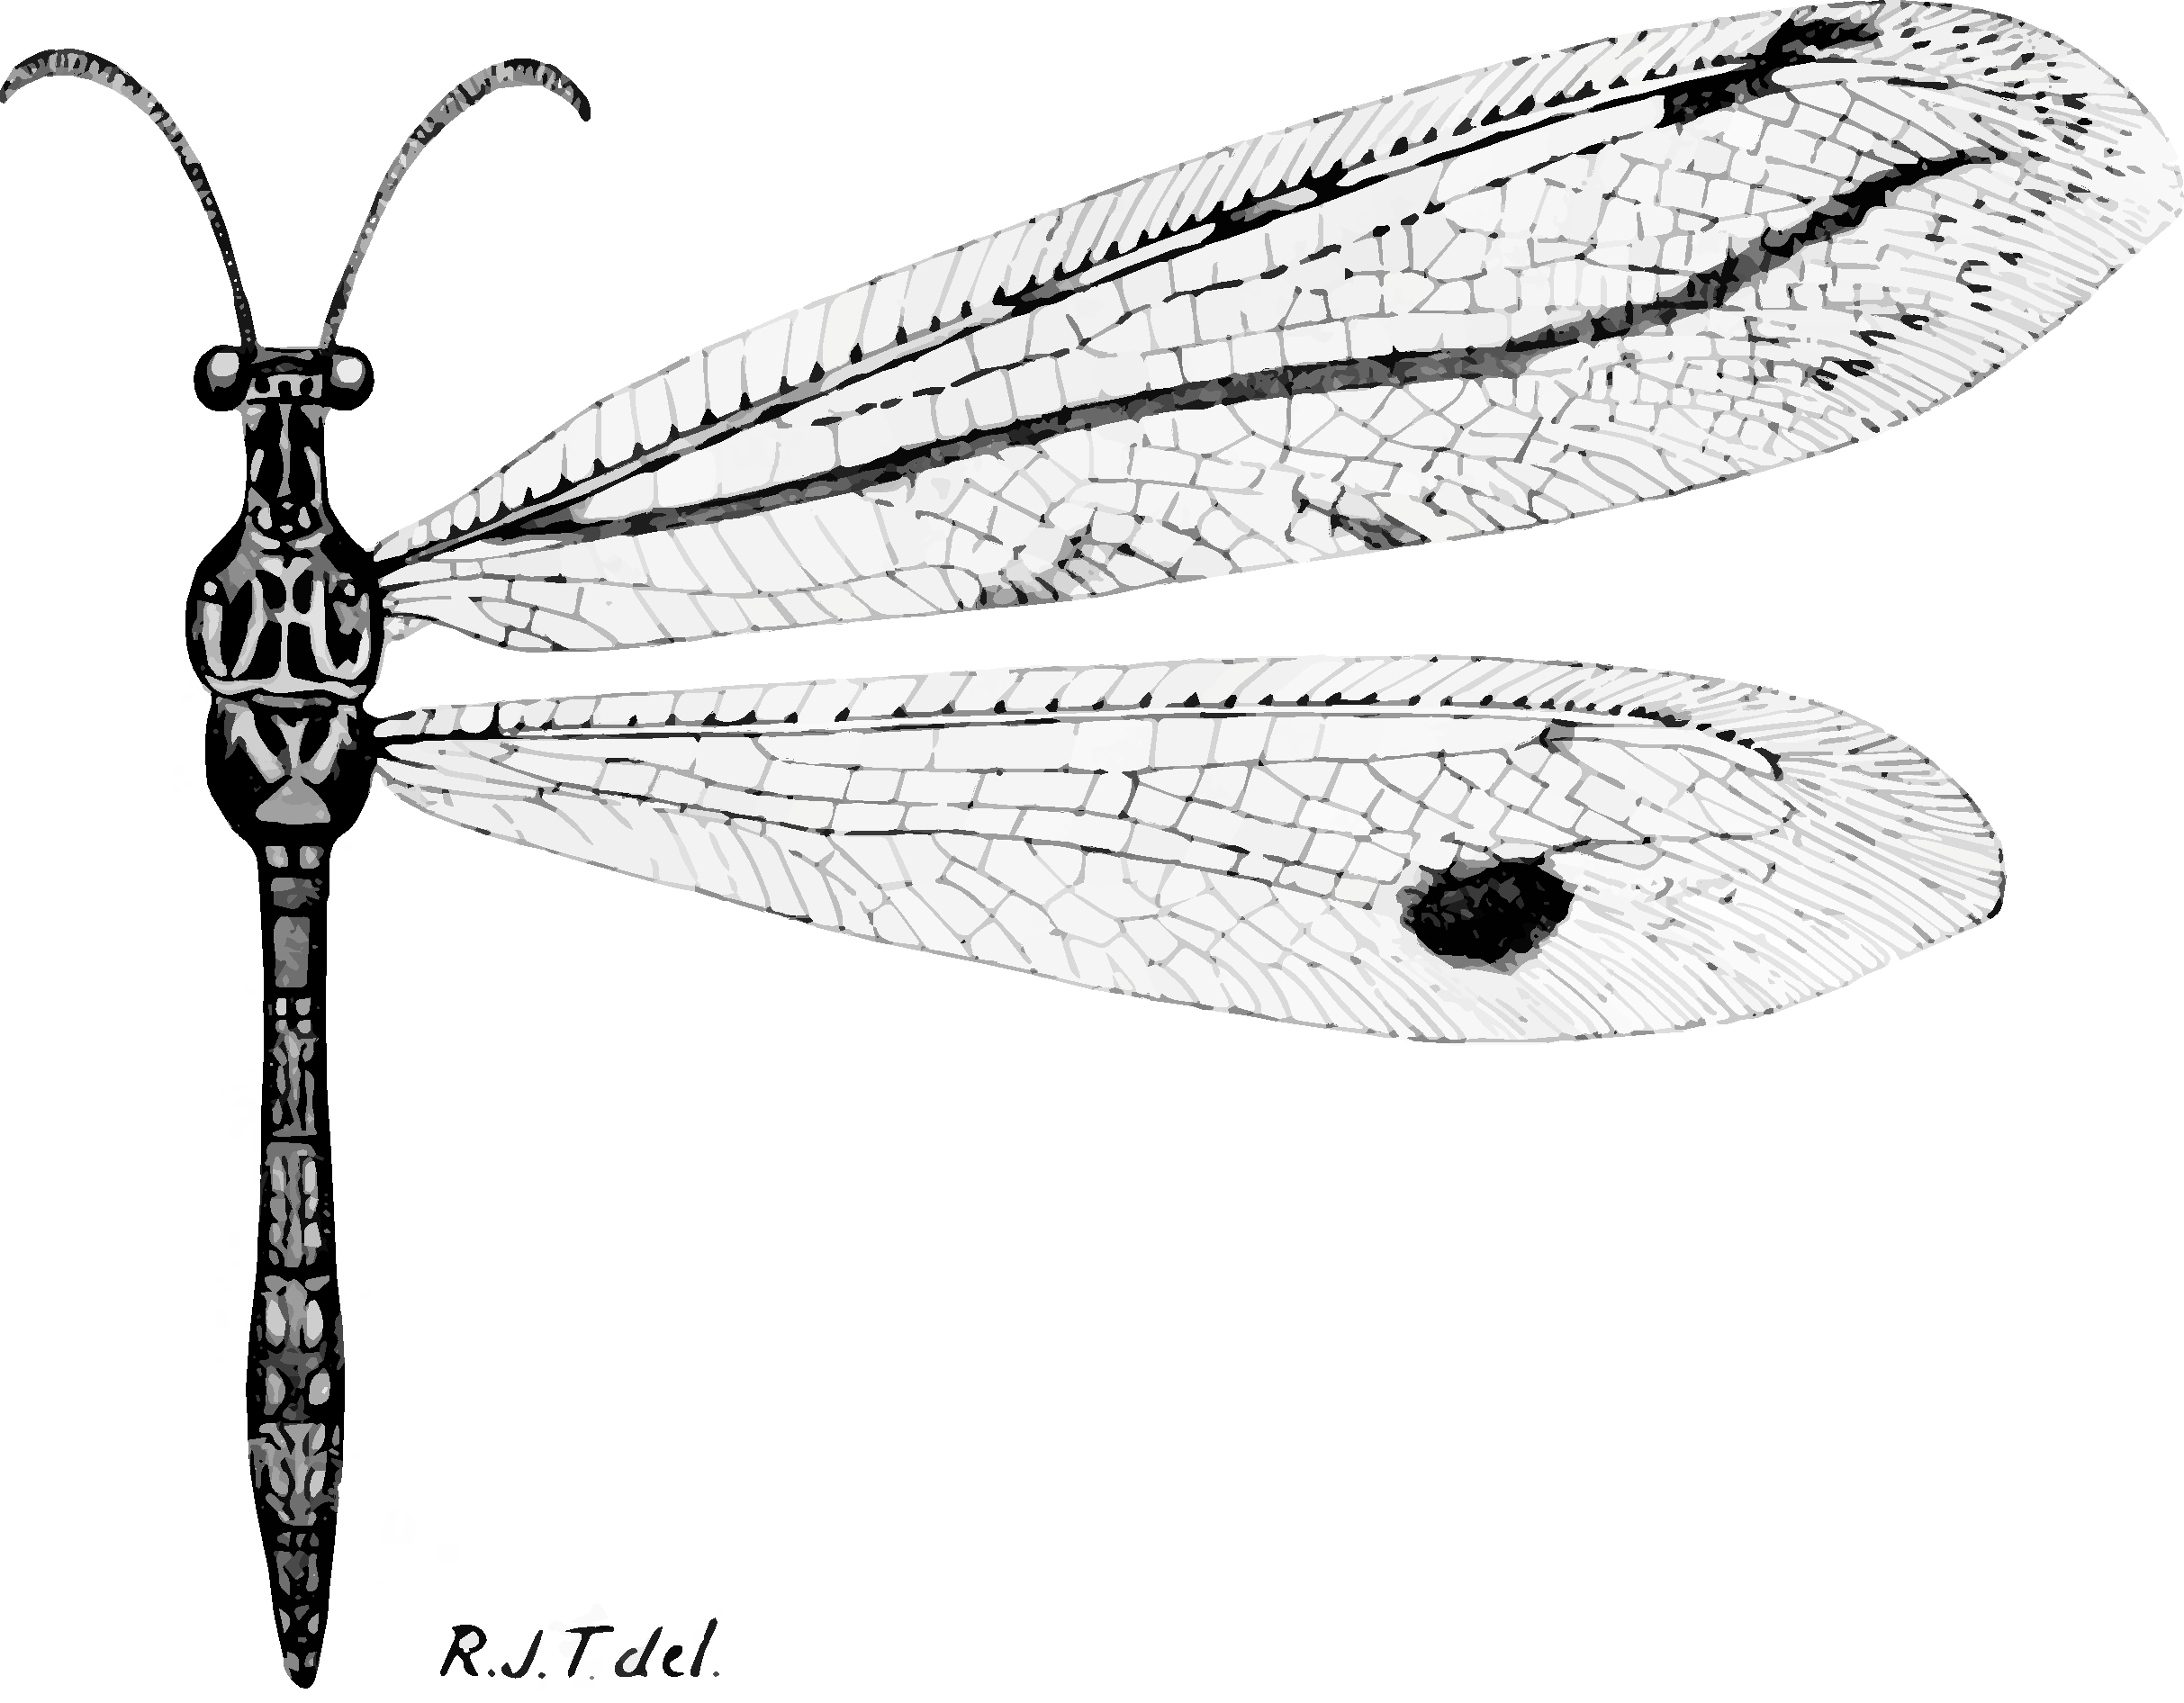
\includegraphics[width=0.46\textwidth]{neuropterida/MyrmeleontidHabitus}
  \caption{Myrmeleontidae habitus \citep[][Fig. III.8]{tillyard1916}}
  \label{fig:myrmeleo}
\end{figure}

\subsubsection{Ascalaphidae (owlflies)}\index{Myrmeleontidae}
\noindent{}\textit{Diagnostic characters:} Antennae clubbed apically, as long as entire body; eyes often divided horizontally into two foveae; thorax often very ``fuzzy''.\vspace{3mm}

\noindent{}\textit{Natural history:} More than 400 species have been described worldwide, and they were recently moved into and then out of Myrmeleontidae. Larvae are ambush predators. Adults are aerial predators that feed similarly to dragonflies.\vspace{3mm}

\begin{figure}[ht!]
  \centering
    \includegraphics[width=0.5\textwidth]{neuropterida/AscalaphidHabitus}
  \caption{Ascalaphidae habitus \citep[modified from][Plate 99]{bhl33187}}
  \label{fig:ascalaph}
\end{figure}

\subsubsection{Chrysopidae (green lacewings)}\index{Chrysopidae}
\noindent{}\textit{Diagnostic characters:} Body color usually dominated by green and/or yellow shades but can be pink, brown, or other colors; antennae thread-like; crossveins along anterior edge of wing unbranched; wing cells tend to be short, boxy (figure \ref{fig:chrysopids}).\vspace{3mm}

\noindent{}\textit{Natural history:} Larvae emerge from stalked eggs and develop as predators of other insects, especially aphids and other soft-bodied insects. Larvae are often referred to as ``aphid wolves'' due to their propensity to cover their bodies in aphid carcasses to avoid detection by prey. Adults consume honeydew and/or other insects as adults. There are at least 1,300 described species worldwide.\vspace{3mm}

\noindent{}\textit{Specimen preparations:} Small adult specimens should ideally be point-mounted, with the tip of the point bent upwards, to fit under the wings. \index[preps]{Chrysopidae}\vspace{3mm}

\begin{figure}[ht!]
  \centering    \includegraphics[width=0.8\textwidth]{neuropterida/chrysopid}
  \caption{Chrysopidae. \textbf{(left)} Dorsal habitus; \textbf{(right)} eggs with hatching larva \citep[modified from][Plate 10, Figs. 1,4]{bhlitem53053}}
  \label{fig:chrysopids}
\end{figure}

\subsubsection{Hemerobiidae (brown lacewings)}\index{Hemerobiidae}
\noindent{}\textit{Diagnostic characters:} Body color almost always mottled brown; antennae thread-like; crossveins along anterior edge of wing branched; wing cells tend to be rectangular/elongate (relative to Chrysopidae).\vspace{3mm}

\noindent{}\textit{Natural history:} Although they are not sister lineages, the natural history of Hemerobiidae is very similar to Chrysopidae; larvae and adults are predators of other insects, especially aphids. There are \textgreater{}600 species wordwide.\vspace{3mm}

\noindent{}\textit{Specimen preparations:} Adult specimens should ideally be point-mounted, with the tip of the point bent upwards, to fit under the wings \index[preps]{Hemerobiidae}

\begin{figure}[ht!]
    \centering
    \begin{subfigure}[ht!]{0.32\textwidth}
        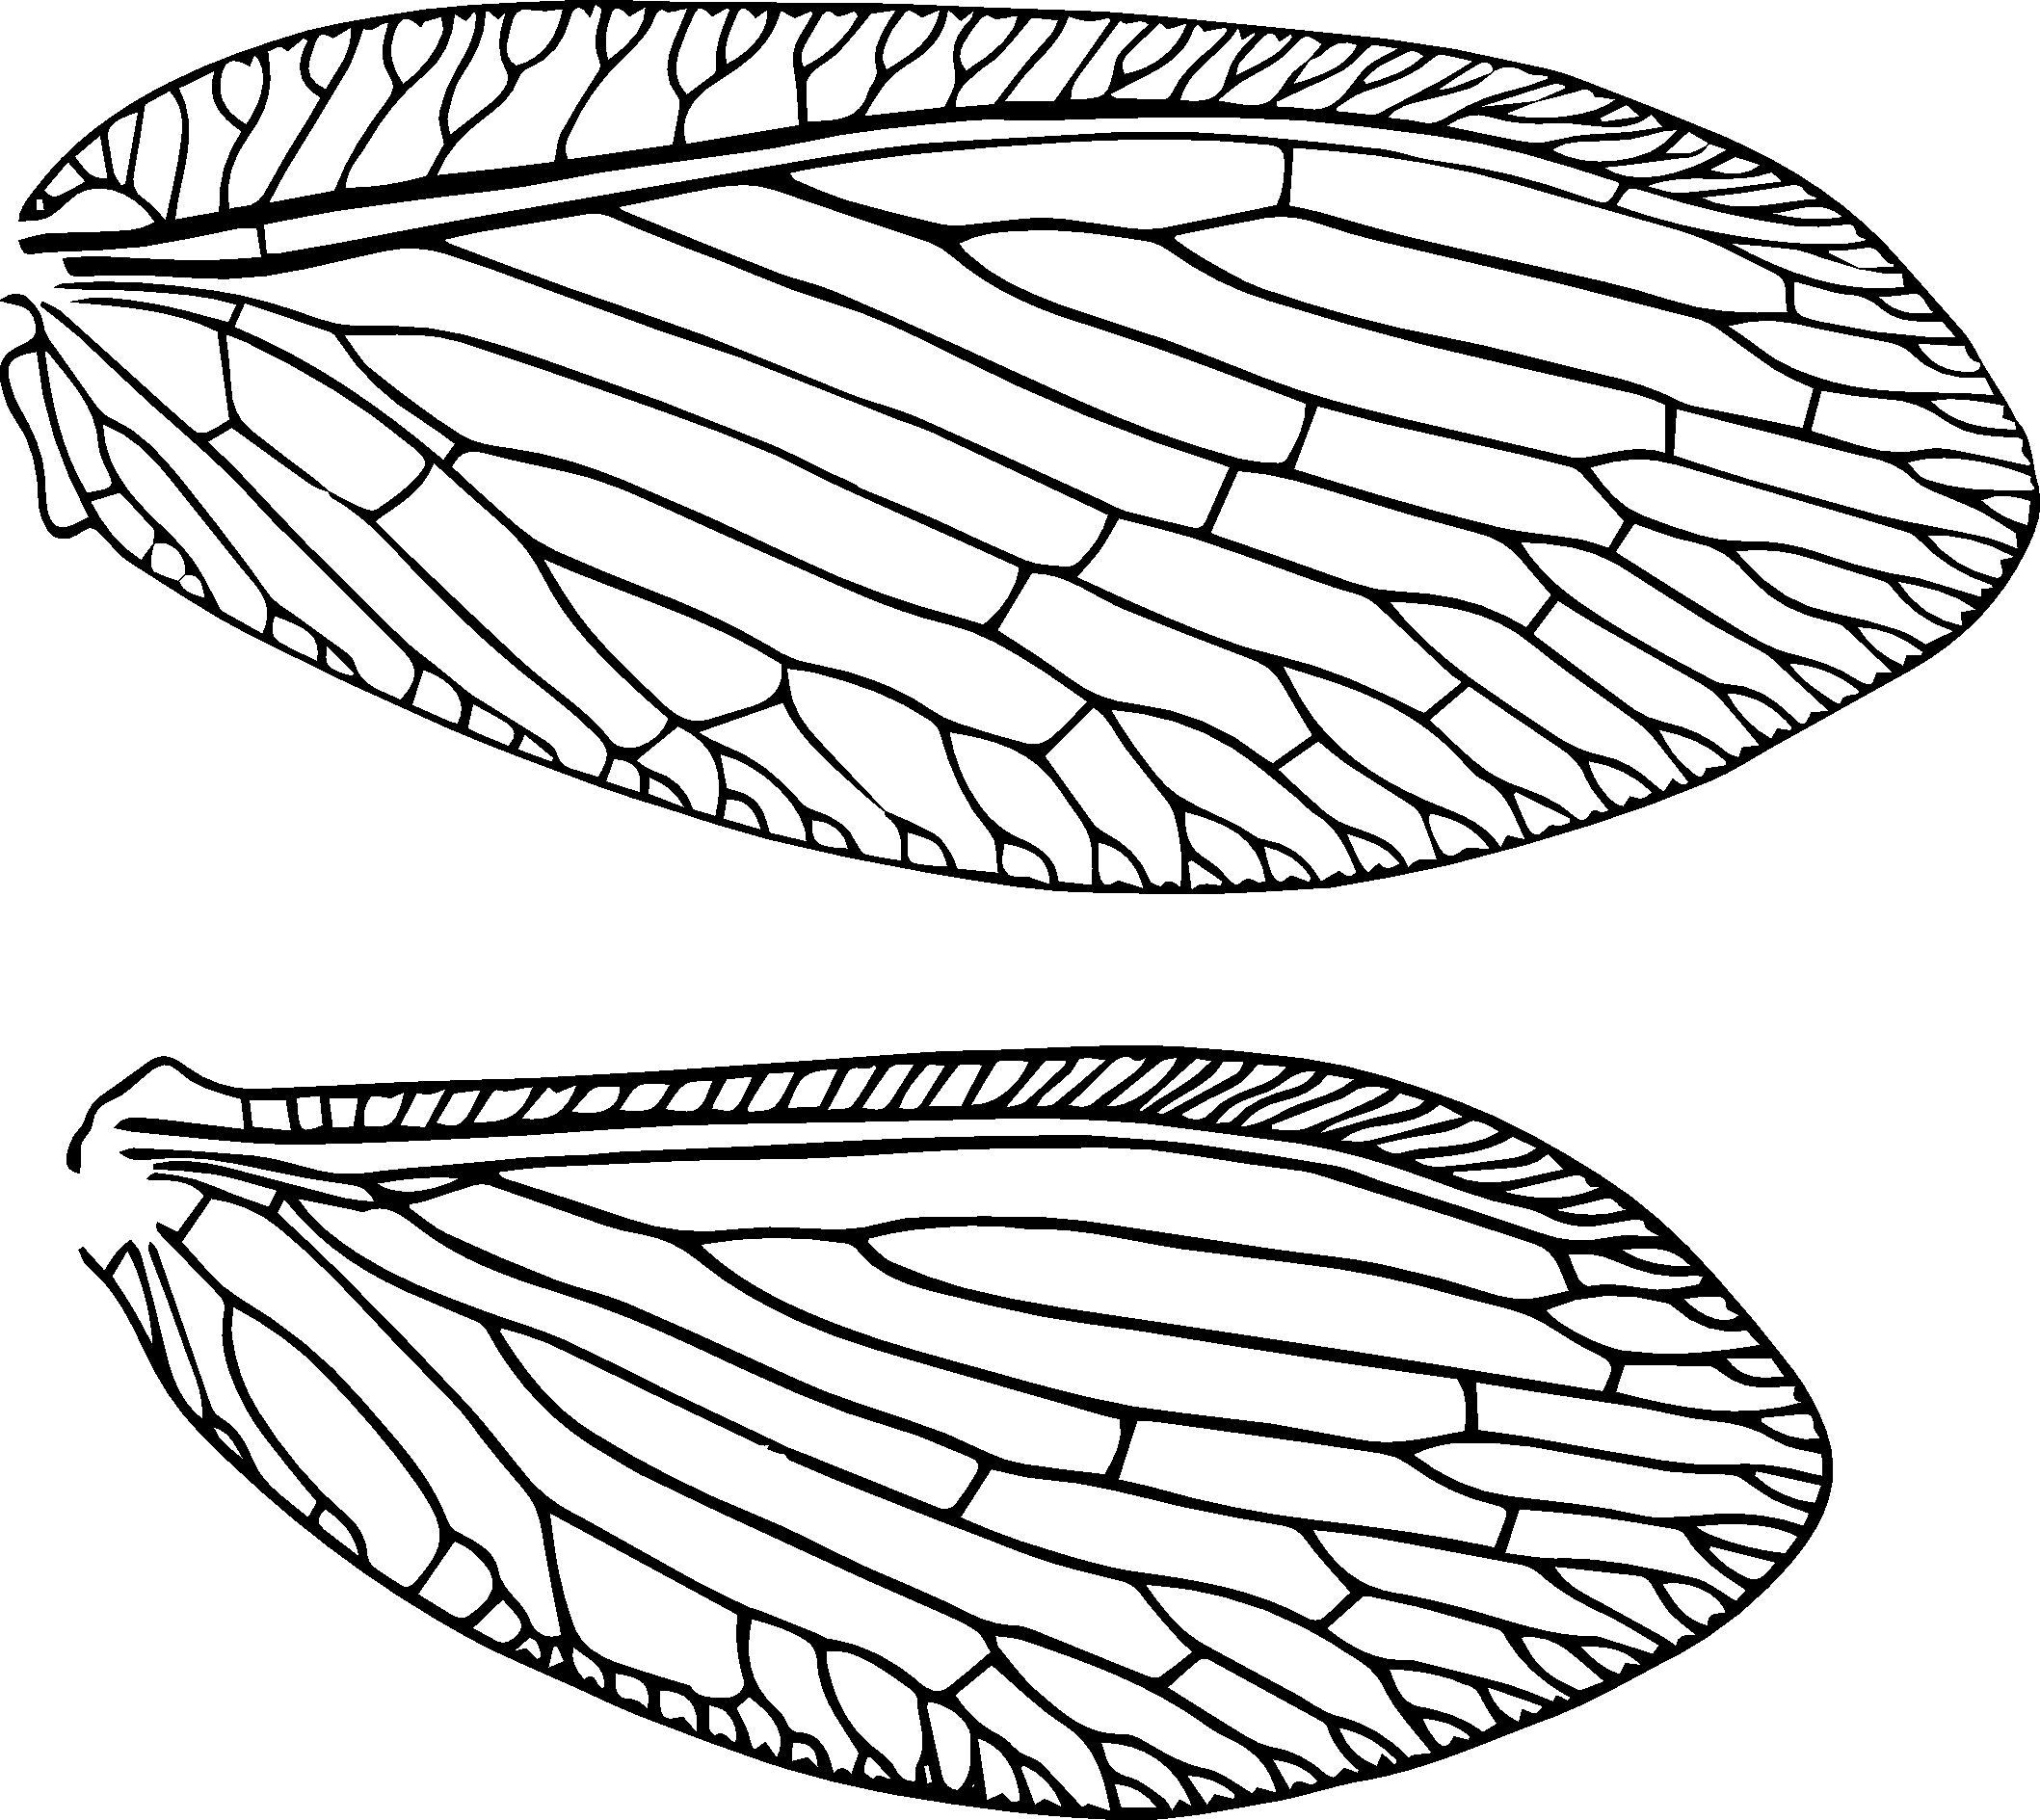
\includegraphics[width=\textwidth]{neuropterida/HemerobiidWing}
        \caption{}
        \label{fig:hemerobiid1}
    \end{subfigure}
    \hfill
    \begin{subfigure}[ht!]{0.58\textwidth}
        \includegraphics[width=\textwidth]{neuropterida/HemerobiidHabitus}
        \caption{}
        \label{fig:hemerobiid2}
    \end{subfigure}
    \caption{Hemerobiidae. \textbf{(a)} Wings \citep[][Fig. 153]{comstock1918wings}; \textbf{(b)} habitus \citep[modified from][Fig. 38]{bhlitem82061AustrInsect}}\label{fig:hemerobiids}
\end{figure}%see also https://www.biodiversitylibrary.org/page/900603

\subsubsection{Mantispidae (mantidflies)}\index{Mantispidae}
\noindent{}\textit{Diagnostic characters:} Antennae relatively short, thread-like; prothorax elongate; fore legs raptorial, arising far anterior on prothorax.\vspace{3mm}

\noindent{}\textit{Natural history:} Larvae often have complex natural histories, \textit{e.g.}, developing as ambush predators in terrestrial habitats, as parasitoids on some Coleoptera and Hymenoptera, or as predators within spider egg sacs. Adults use raptorial fore legs to catch prey, and many species mimic stinging Hymenoptera.\vspace{3mm}

\begin{theo}
{}How are these insects different than mantids? How are they the same?
\end{theo}

\begin{figure}[ht!]
  \centering
    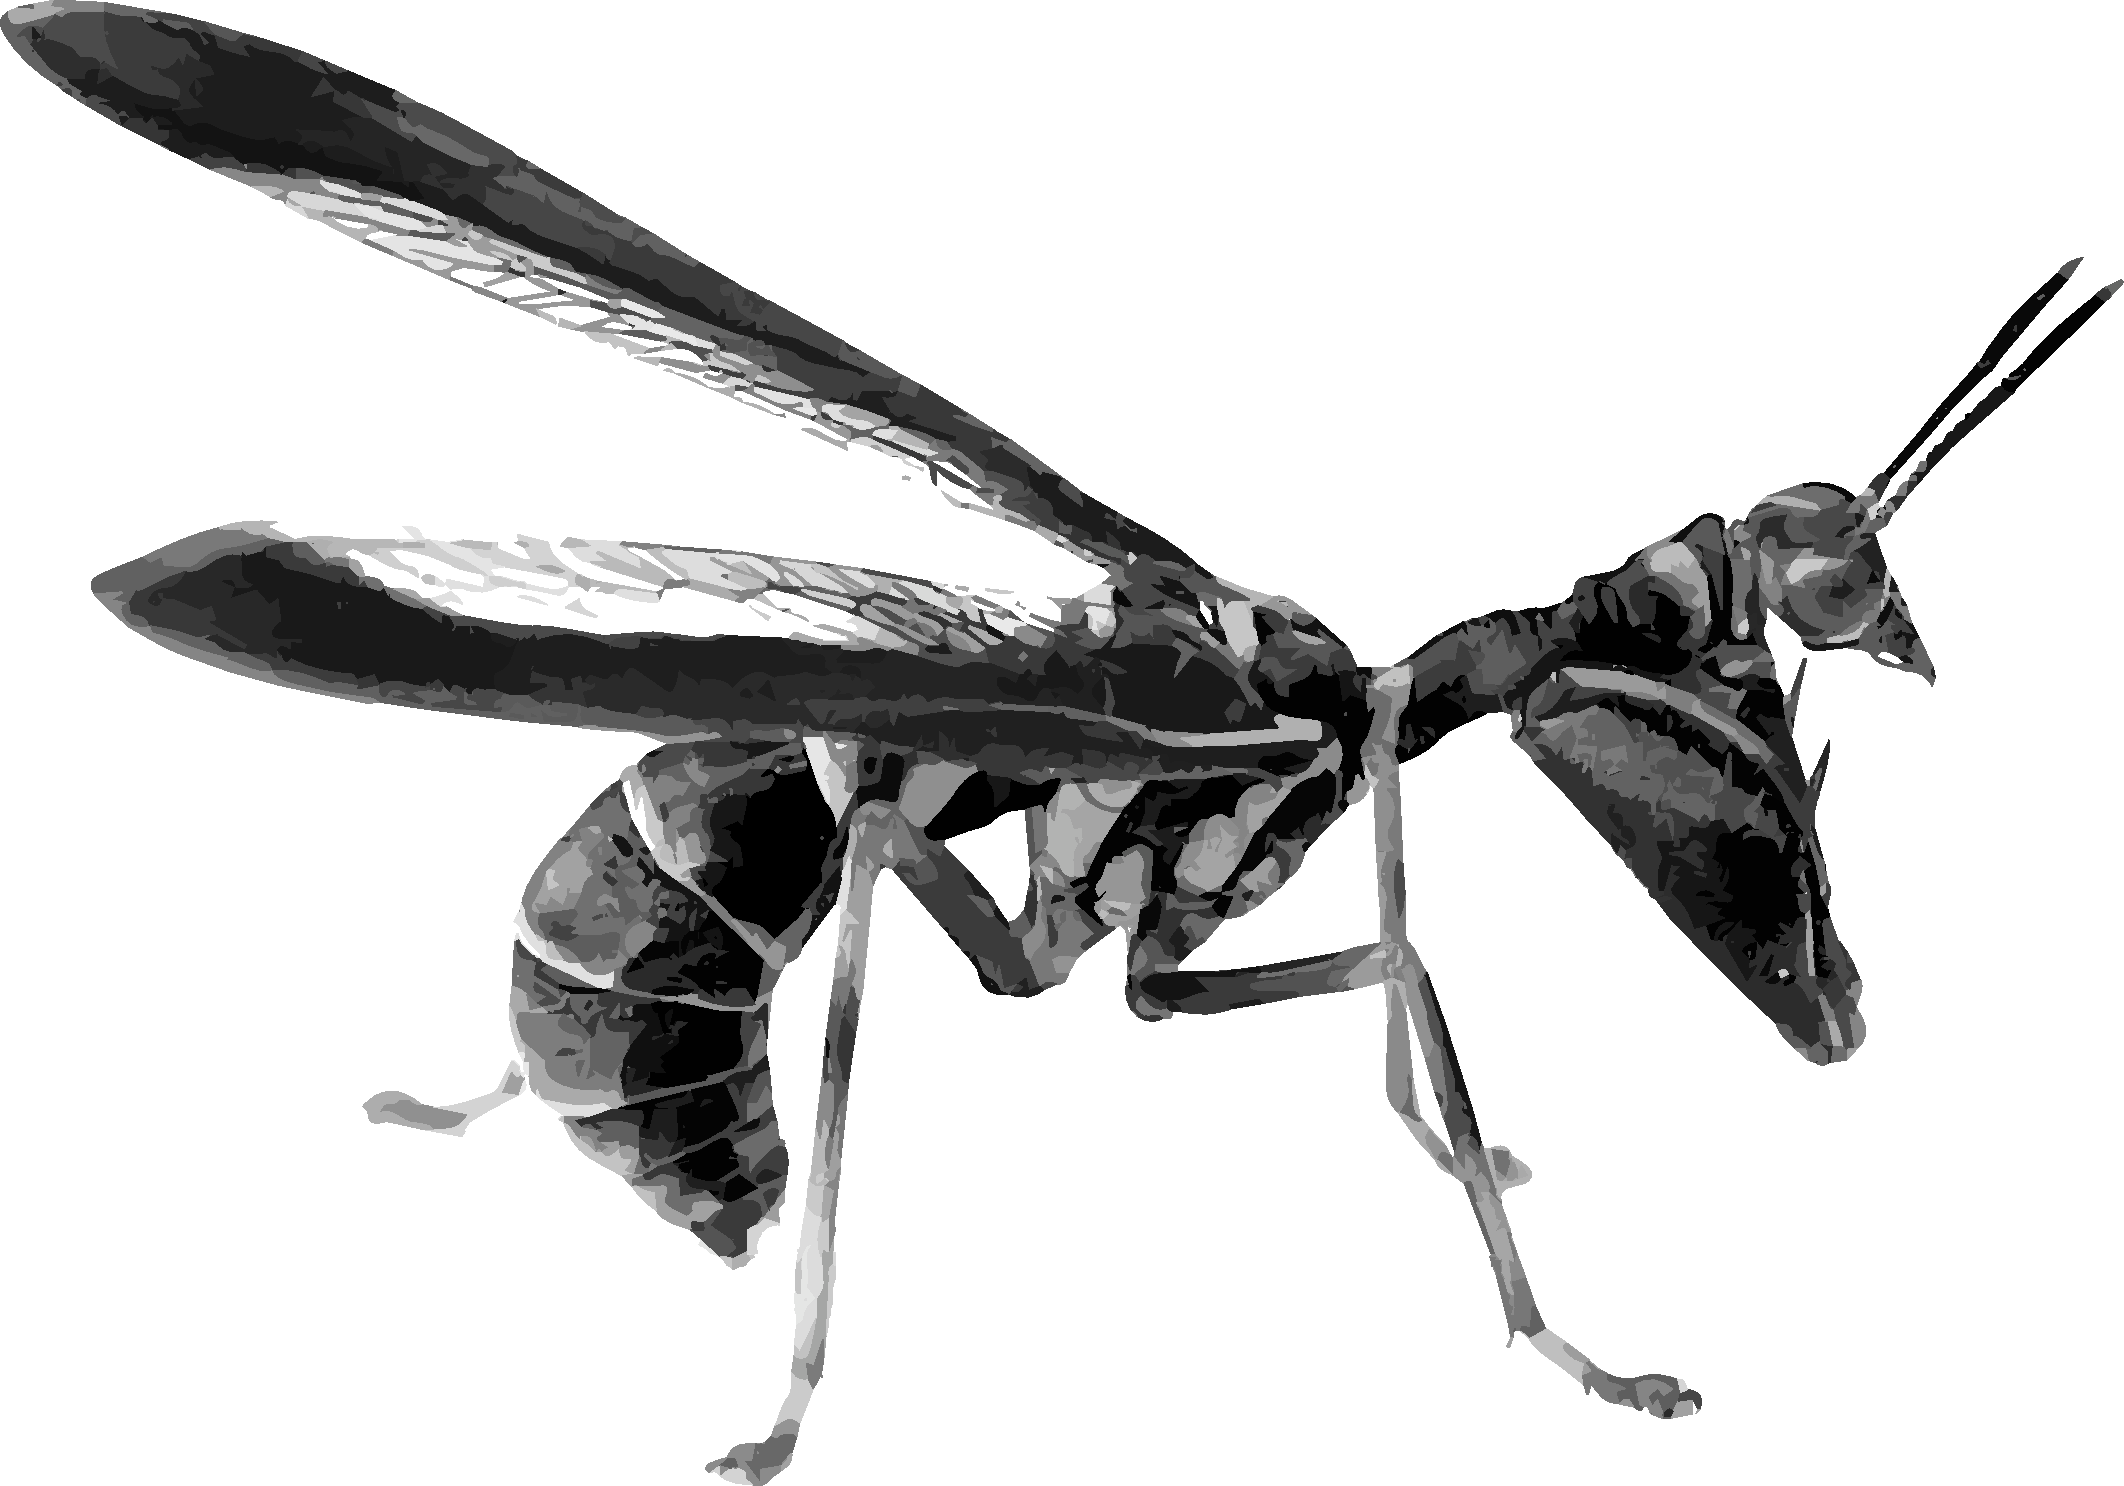
\includegraphics[width=0.45\textwidth]{neuropterida/MantispidHabitus}
  \caption{Mantispidae habtus. Redrawn from photo (CC BY-SA 3.0 unported) by Ilona Loser, via Wikimedia Commons}
  \label{fig:mantispid}
\end{figure}%https://www.biodiversitylibrary.org/page/900343

\subsubsection{Coniopterygidae (dustywings)}\index{Coniopterygidae}
\noindent{}\textit{Diagnostic characters:} Body much smaller (usually \textless7 mm) than most other neuropterans and covered in white waxy substance; wings with fewer veins than other neuropterans (\textit{e.g.}, R branches only twice; figure \ref{fig:coniopterygid1}).\vspace{3mm}

\noindent{}\textit{Natural history:} Larvae live on woody plants, where they eat small, soft-bodied prey---including whiteflies (Aleyrodidae) and mealybugs (Pseudococcidae), to which dustywings have more than a passing resemblance. There are almost 500 species known worldwide.\vspace{3mm}

\noindent{}\textit{Specimen preparations:} Adult specimens should be double- or slide-mounted \index[preps]{Coniopterygidae}

\begin{theo}
{}Why are some insects, like Coniopterygidae, covered in a waxy powder? What are the possible functions of this substance, which can be found on larvae and adults.
\end{theo}

\begin{figure}[ht!]
    \centering
    \begin{subfigure}[ht!]{0.32\textwidth}
        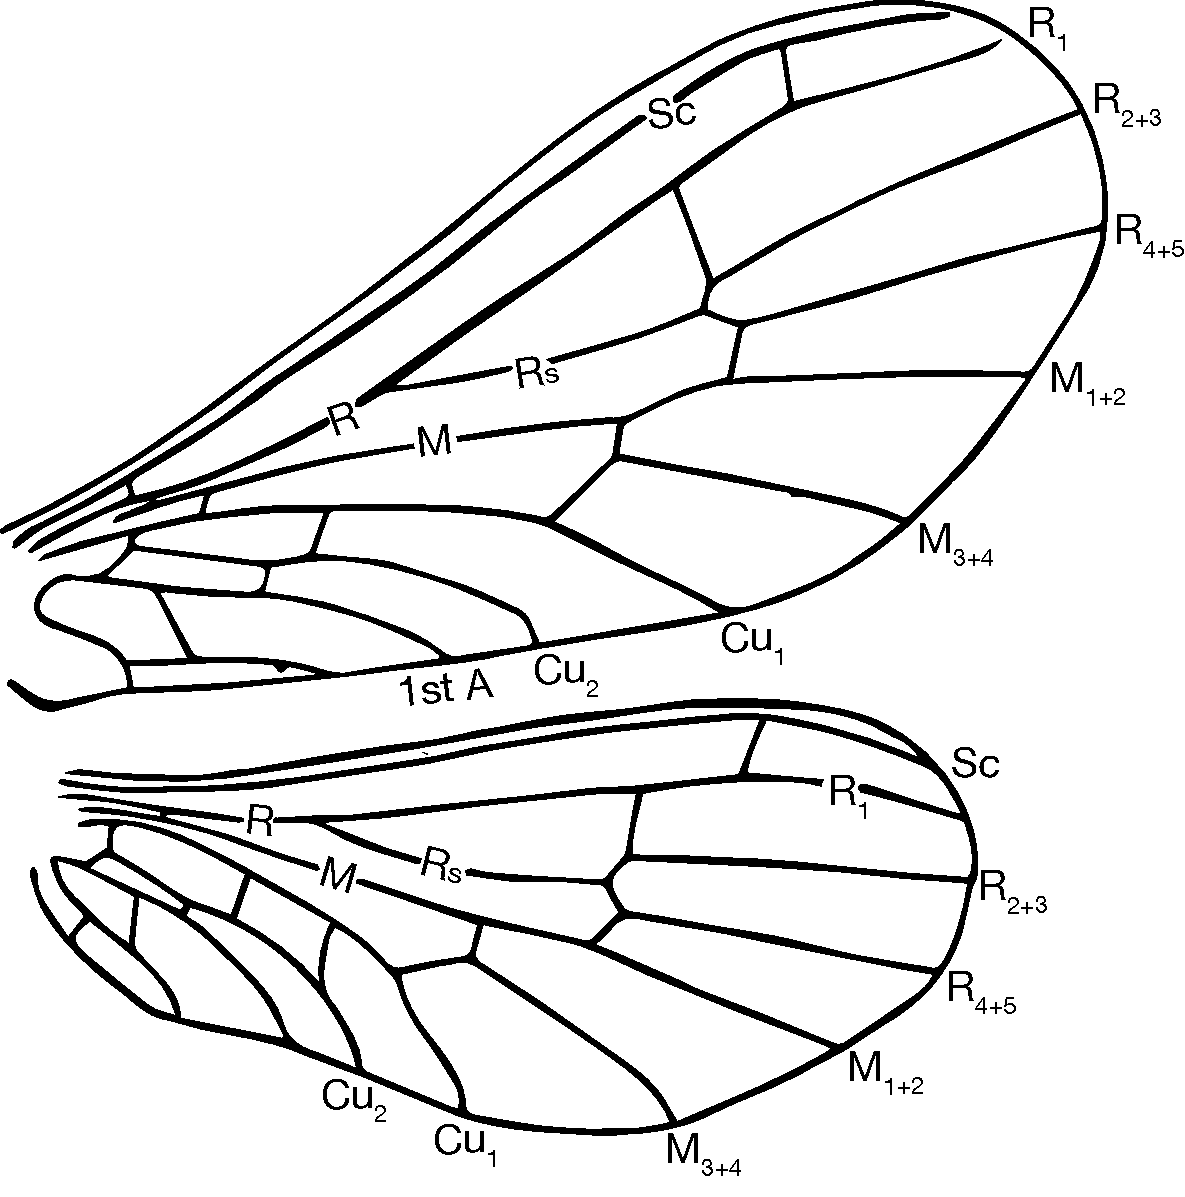
\includegraphics[width=\textwidth]{neuropterida/ConiopterygidWing}
        \caption{}
        \label{fig:coniopterygid1}
    \end{subfigure}
    \qquad
    \begin{subfigure}[ht!]{0.48\textwidth}
        \includegraphics[width=\textwidth]{neuropterida/ConiopterygidHabitus}
        \caption{}
        \label{fig:coniopterygid2}
    \end{subfigure}
    \caption{Coniopterygidae. \textbf{(a)} Wings \citep[][Fig. 211]{comstock1918wings}; \textbf{(b)} habitus, photo (CC BY 3.0) by BartBotje (source: Wikimedia Commons)}\label{fig:coniopterygids}%need line drawing or black and white
\end{figure}
\FloatBarrier

\section{Raphidioptera (snakeflies)}\index{Raphidioptera}
The prothorax elongate but legs arise posteriorly on prothorax. In North America, these insects are found only out west.\vspace{3mm}

\subsubsection{Raphidiidae}\index{Raphidiidae}
\noindent{}\textit{Diagnostic characters:} Female with long ovipositor; ocelli present; crossvein present inside stigma.\vspace{3mm}

\noindent{}\textit{Natural history:} All stages are predaceous, and one can usually find these insects near or on trees.\vspace{3mm}

\begin{figure}[ht!]
  \centering
    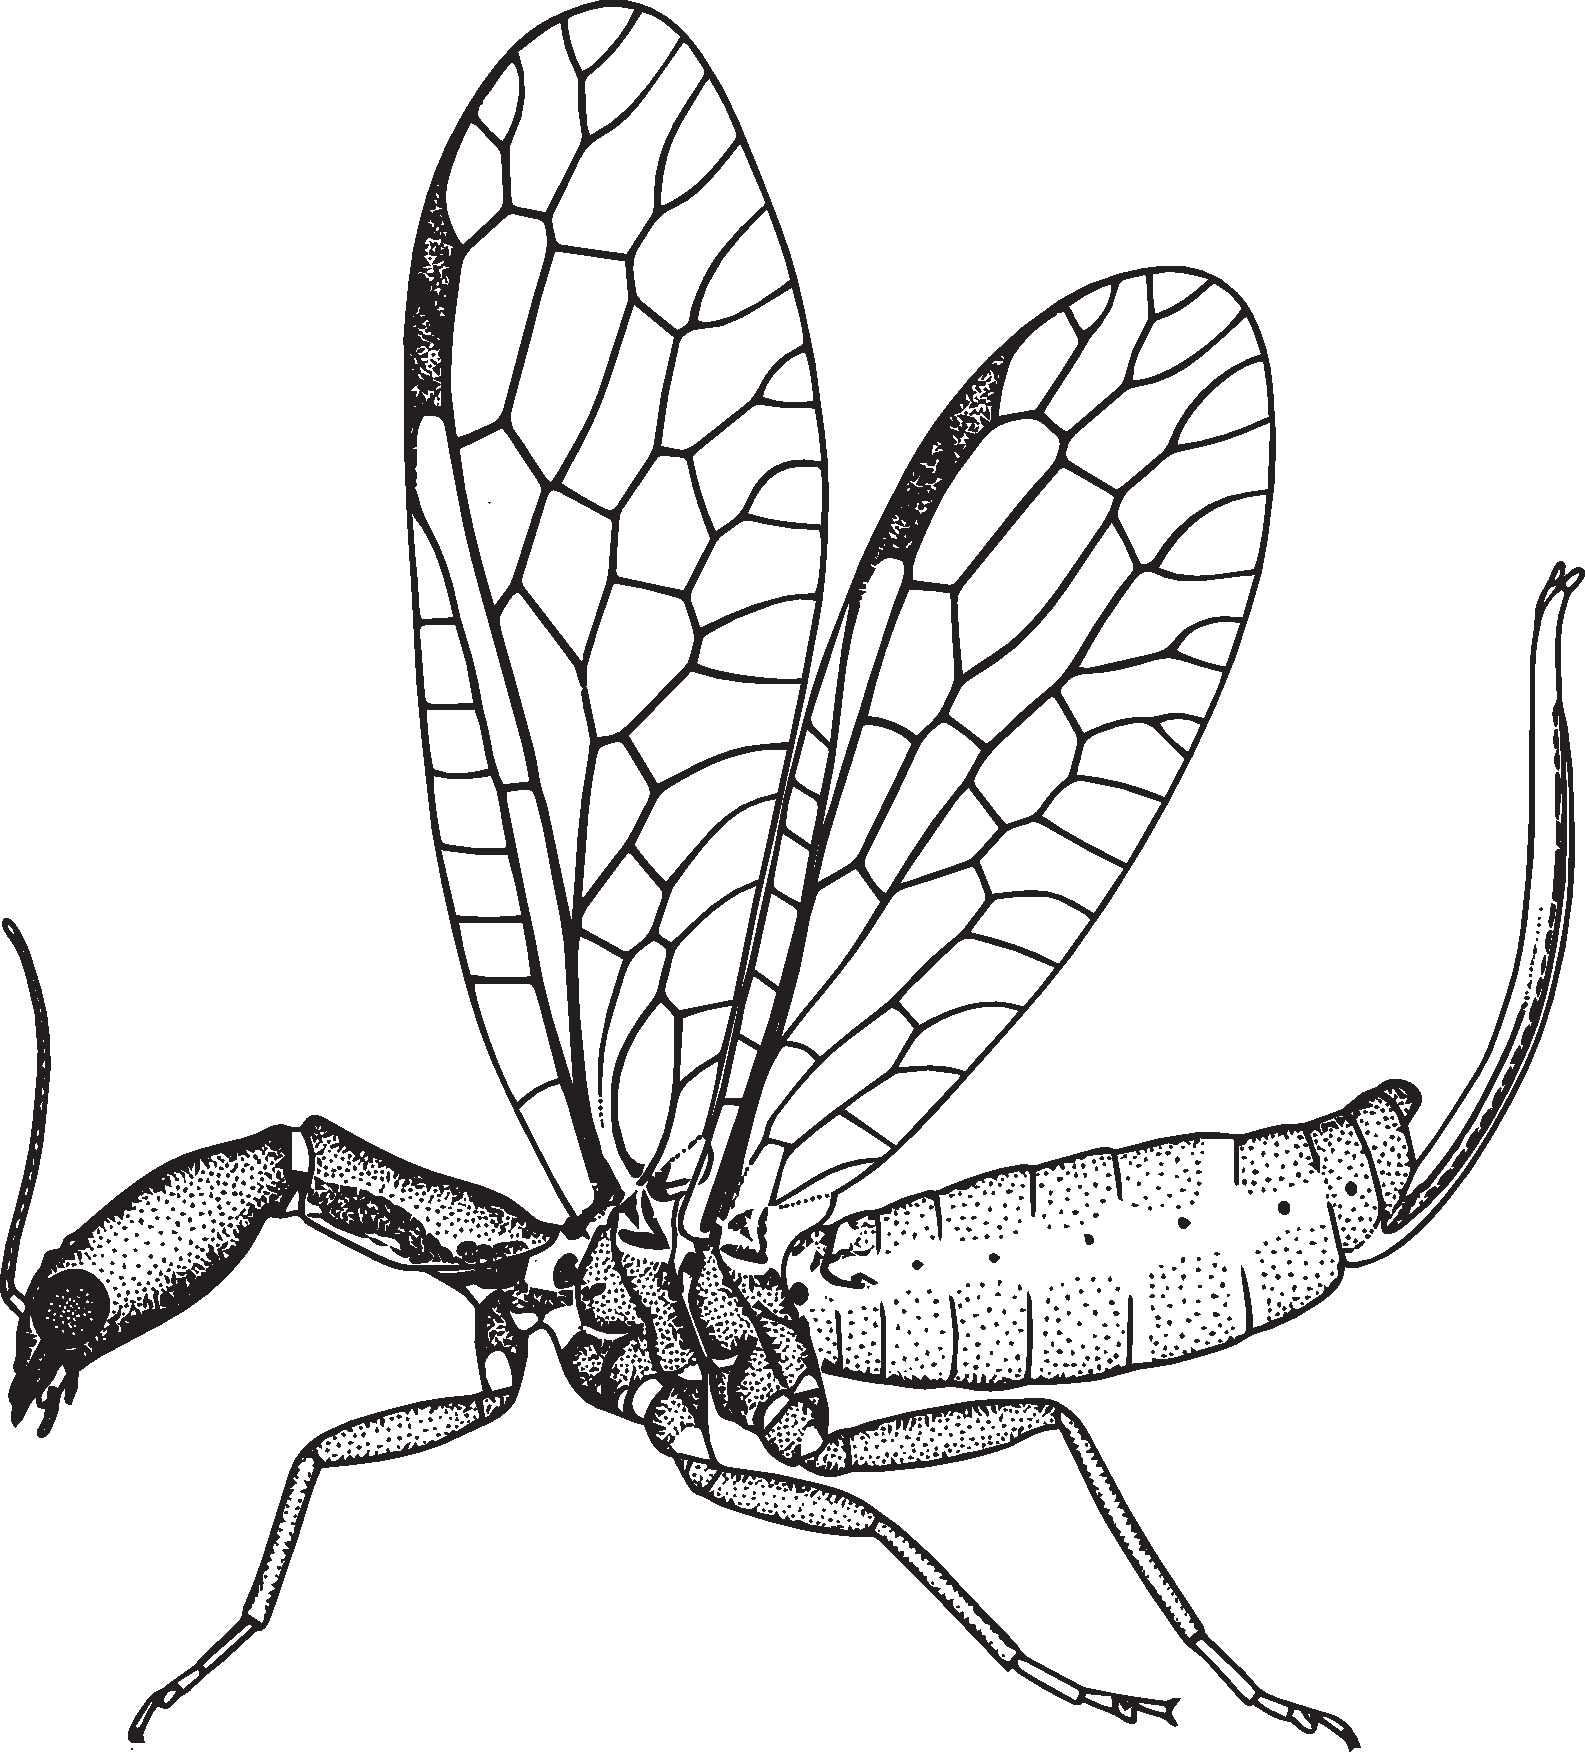
\includegraphics[width=0.38\textwidth]{neuropterida/raphidiidHabitus}
  \caption{Raphidiidae. Adapted from drawing by Nikita Kluge (CC0; source: \url{https://commons.wikimedia.org/})}
  \label{fig:raphid}
\end{figure}

\section*{Test yourself}
This lineage is usually referred to as relictual. What does that mean? Why are these insects perhaps less diverse now than they were millions of years ago?\vspace{3mm}

\noindent{}All known species are predators. Can you describe two or three adaptations these insects have for hunting, capturing, and otherwise subduing prey?\vspace{3mm}

\noindent{}Familiarize yourself with the following taxon names, which refer to organisms you are likely to encounter in the northeastern USA and/or which are phylogenetically relevant. Can you describe how these arthropods live (natural history) and roughly how diverse they are? Do you know how they're related to one another? If you had to choose a family to study from the taxa below which one would it be and why?
\begin{enumerate} 
\item Neuroptera  
\item Megaloptera
\item Raphidioptera
\end{enumerate}

\clearpage
\thispagestyle{empty}